\chapter[\crcszeroshorttitle{}]{\crcszerolongtitle{}}

\label{crcs0}


\section{Introduction}

\index{ratiometric conversion and calculation}
This chapter describes the construction and analysis of ratiometric conversion and
measurement systems.  By \emph{ratiometric}, we mean that the system requires input
from multiple A/D channels to infer the data of interest, typically a potentiometer
position.  Ratiometric conversion and calculation systems are most often used in
small microcontroller work because they can reduce cost by eliminating regulated
voltage supplies.  Successive sections in the chapter describe the analysis of progressively
more complex ratiometric conversion and calculation systems.


\section{Ratiometric Conversion In Hardware Versus Ratiometric Calculation In Software}

Need to include a differentiation between conversion in hardware and
calculation in software.


%Section tag: srsy1
%
\section{Potentiometer With $V_{+}$ Reference And Hardware Ratiometric Conversion}

The simplest ratiometric potentiometer system
that would be constructed in practice
is shown in Fig. \ref{crcs0:srsy1:smplsys0}.
In this system, microcontroller software must sense
the potentiometer position $R_{P1}/R_P$\footnote{We hope that
all of our readers have a background that allows them to
analyze resistor networks.  For readers without this background,
we recommend reading and working through the exercises in an
undergraduate circuit analysis text.} even as
$V_{+}$ varies within the interval
$V_{+} \in [V_{+MIN}, V_{+MAX}]$.  Such systems, with
additional filtering and current-limiting components,
are commonly used in automobiles to allow a microcontroller
software load to sense seat or
mirror position.
\index{seat position}
\index{mirror position}
\index{battery voltage}
Using automobile battery voltage as $V_{+}$
has the advantage that a regulated voltage is not
required, thus saving the component cost and circuit board
area of a voltage regulator.

\begin{figure}[!tb]
\centering
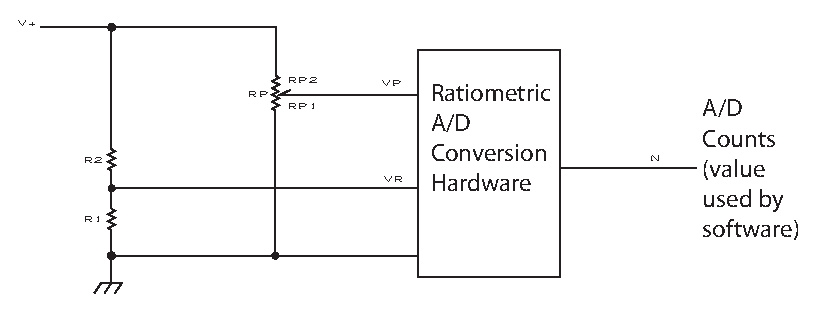
\includegraphics[width=4.6in]{c_rcs0/s_rsy1/smplsys0.eps}
\caption{Simple Ratiometric Measurement System With Hardware Ratiometric Conversion}
\label{crcs0:srsy1:smplsys0}
\end{figure}

In the circuit of Fig. \ref{crcs0:srsy1:smplsys0}, the microcontroller
\index{A/D converter}A/D converter will convert $V_P$ using $V_R$ as a voltage
reference according to the relationship in (\ref{crcs0:srsy1:eq000}), where $N_{MAX}$
is the maximum count of the A/D converter.  The \index{floor function}$floor(\cdot{})$
function in (\ref{crcs0:srsy1:eq000}) is used to model the effect of
\index{quantization}quantization---the
A/D count $N$ is required to be $\in \vworkintsetnonneg$.

\begin{equation}
\label{crcs0:srsy1:eq000}
N = \left\lfloor { \frac{N_{MAX} V_P}{V_R} } \right\rfloor
\end{equation}



%Section tag: srsy0
%
\section{Fixed $r_{1}$, Fixed $r_{2}$ System}
The simplest ratiometric system that would be constructed in practice
is shown in Fig. \ref{crcs0:srsy0:fr1fr2a}.
In Fig. \ref{crcs0:srsy0:fr1fr2a},
assume that the potentiometer is positioned so that
$R_{P1}$ is the resistance from the potentiometer wiper
to ground, and $R_{P2}$ is the resistance from the potentiometer
wiper to $V_{+}$.  By definition, $R_{P} = R_{P1} + R_{P2}$.  $z_R$ and
$z_P$ are the transfer coefficients which relate voltage to A/D counts.
These transfer coefficients are an analysis convenience, and correspond to
A/D converter characteristics.

\begin{figure}[!tb]
\centering
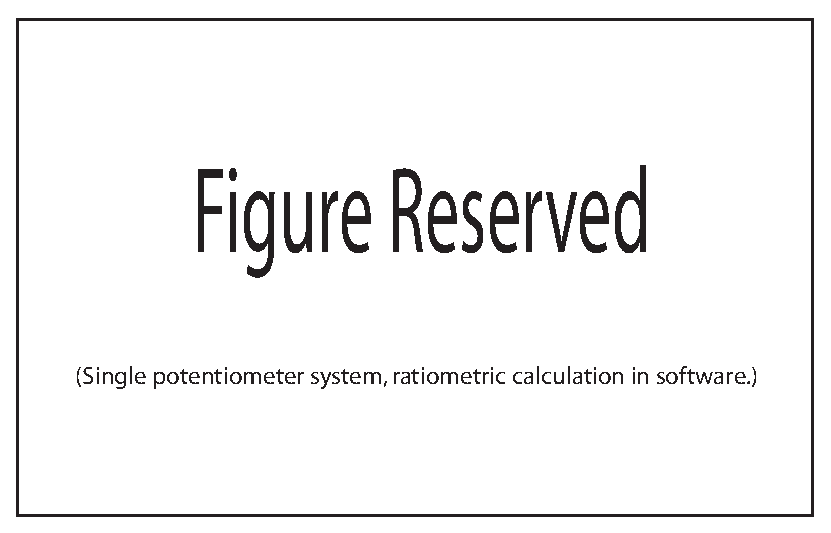
\includegraphics[height=2.5in]{c_rcs0/s_rsy0/smplsys0.eps}
\caption{Simple Ratiometric Measurement System With Software Ratiometric Calculation}
\label{crcs0:srsy0:fr1fr2a}
\end{figure}

The circuit is designed to allow
estimation of $R_{P1}$ (effectively, the potentiometer position)
under conditions of varying $V_{+}$.  The economy of such a circuit
comes from the characteristic that $V_{+}$ need not be regulated,
thus allowing less expensive lower-capacity voltage regulators or
fewer voltage regulators to be used in an embedded system.
In an vehicle, for example, $V_{+}$ may be the battery voltage of
the vehicle, which will vary substantially based on which
electrical loads are turned on, whether the starter motor is
engaged, etc.

The critical analysis question is,
how accurately can $R_{P1}/R_P$ be estimated under conditions
of varying $V_{+} \in [V_{+MIN}, V_{+MAX}]$?  Or, equivalently,
given measured values of $y_R, y_P \in \vworkintsetnonneg$
and given $V_{+} \in [V_{+MIN}, V_{+MAX}]$,
what inequality describes the possible values of $R_{P1}/R_P$
(i.e. how much can be inferred or implied from the observation)?


From analysis of the circuit of Fig. \ref{crcs0:srsy0:fr1fr2a},
it can be shown that (\ref{crcs0:srsy0:eq000}) applies.
However, because an A/D
count is necessarily $\in \vworkintsetnonneg$, (\ref{crcs0:srsy0:eq000b}) must be
used for analysis.

\begin{equation}
\label{crcs0:srsy0:eq000}
y_R = \frac{R_1 z_R V_{+}}{R_1 + R_2}
\end{equation}

\begin{equation}
\label{crcs0:srsy0:eq000b}
y_R = \left\lfloor\frac{R_1 z_R V_{+}}{R_1 + R_2}\right\rfloor
\end{equation}

Similarly, (\ref{crcs0:srsy0:eq000c}) describes $y_P$ for analysis.

\begin{equation}
\label{crcs0:srsy0:eq000c}
y_P = \left\lfloor\frac{R_{P1} z_R V_{+}}{R_P}\right\rfloor
\end{equation}


\section{Unplaced Equations}

This section is a holding place for equations until can get my
thoughts together.

\begin{equation}
y_P = \frac{R_{P1}}{R_P} V_{+}
\end{equation}

\begin{equation}
V_{+} = y_P \left( {\frac{R_P}{R_{P1}}} \right)
\end{equation}

\begin{equation}
y_R = \frac{R_1}{R_1 + R_2} V_{+}
\end{equation}

\begin{equation}
V_{+} = \frac{y_R ( R_1 + R_2)}{R_1}
\end{equation}

\begin{equation}
y_P \left( {\frac{R_P}{R_{P1}}} \right) = y_R \left( {\frac{R1 + R2}{R1}} \right)
\end{equation}

\begin{equation}
\frac{R_P}{R_{P1}} = \frac{y_R}{y_P} \left( {\frac{R_1 + R_2}{R_1}} \right)
\end{equation}

\begin{equation}
\frac{R_{P1}}{R_P} = \frac{y_P}{y_R} \left( {\frac{R_1}{R_1 + R_2}} \right)
\end{equation}

\begin{equation}
\frac{R_P V}{R_P V + 1} < \frac{\lfloor R_P V \rfloor}{\lfloor R_R V \rfloor} < \frac{R_P V + 1}{R_R V}
\end{equation}

%%%%%%%%%%%%%%%%%%%%%%%%%%%%%%%%%%%%%%%%%%%%%%%%%%%%%%%%%%%%%%%%%%%%%%%%%%
%End of file c_rcs0.tex

